\ifdefined\inMainDoc\else
\documentclass[12pt,a4paper]{article}
% ================================================================
%  PRÉAMBULE COMMUN - ANNALES CORRIGÉES
%  Université de Kara - FaST - Licence Fondamentale MPC
%  Design optimisé impression noir et blanc
% ================================================================

% -- ENCODAGE & LANGUE --
\usepackage[utf8]{inputenc}
\usepackage[T1]{fontenc}
\usepackage[french]{babel}
\usepackage{lmodern}
\usepackage{microtype}

% -- MISE EN PAGE --
\usepackage[a4paper, top=2.8cm, bottom=2.5cm, left=2.5cm, right=2.5cm, headheight=14pt]{geometry}
\usepackage{setspace}
\setstretch{1.2}
\usepackage{parskip}
\setlength{\parindent}{1.2em}
\setlength{\parskip}{4pt}

% -- MATHS --
\usepackage{amsmath, amssymb, mathtools, amsthm}
\usepackage{mathrsfs}
\usepackage{dsfont}
\usepackage{bm}
\usepackage{cancel}
\usepackage{textcomp}
% Définition de \oiint (intégrale de surface fermée) sans package supplémentaire
\newcommand{\oiint}{\mathop{\iint\!\!\!\!\!\!\!\bigcirc}\limits}

% -- PHYSIQUE & CHIMIE --
\usepackage{physics}
\usepackage{siunitx}
% Lorsque physics est chargé, siunitx omet \qty. On le restaure ici :
\AtBeginDocument{\RenewCommandCopy\qty\SI}
\sisetup{locale = FR, detect-all, output-decimal-marker={,}}
% Commande de substitution pour les unités posant problème avec pdflatex
% (ohm, degreeCelsius, micro, angstrom, percent utilisent des caractères non-ASCII)
\newcommand{\qtyohm}[1]{\ensuremath{\num{#1}\,\Omega}}
\newcommand{\qtydegc}[1]{\ensuremath{\num{#1}\,{}^\circ\text{C}}}
\newcommand{\qtyangstrom}[1]{\ensuremath{\num{#1}\,\text{\AA}}}
\newcommand{\qtypercent}[1]{\ensuremath{\num{#1}\,\%}}
\newcommand{\qtyum}[1]{\ensuremath{\num{#1}\,\mu\text{m}}}
\usepackage[version=4]{mhchem}

% -- GRAPHISMES --
\usepackage{graphicx}
\usepackage{float}
\usepackage{caption}
\usepackage{subcaption}
\usepackage{wrapfig}
\usepackage{tikz}
\usetikzlibrary{calc, arrows.meta, patterns, shapes.geometric}
\usepackage{pgfplots}
\pgfplotsset{compat=1.18}

% -- TABLEAUX --
\usepackage{booktabs}
\usepackage{array}
\usepackage{tabularx}
\usepackage{multirow}

% -- LISTES --
\usepackage{enumitem}
\setlist[enumerate]{topsep=3pt, itemsep=2pt, parsep=0pt}
\setlist[itemize]{topsep=3pt, itemsep=2pt, parsep=0pt, label={.}}

% -- BOÎTES (noir et blanc) --
\usepackage{mdframed}
\usepackage{tcolorbox}
\tcbuselibrary{skins, breakable, theorems}

% Boîte EXERCICE : encadré avec filet épais, fond blanc
\newmdenv[
  linewidth=1.2pt,
  linecolor=black,
  roundcorner=3pt,
  skipabove=10pt,
  skipbelow=6pt,
  innertopmargin=8pt,
  innerbottommargin=8pt,
  innerleftmargin=10pt,
  innerrightmargin=10pt,
  backgroundcolor=white,
  frametitle={\bfseries\small Exercice},
  frametitlealignment=\raggedright,
  frametitleaboveskip=4pt,
  frametitlebelowskip=4pt,
]{boiteexercice}

% Boîte CORRIGÉ : fond gris très clair + filet fin
\newmdenv[
  linewidth=0.6pt,
  linecolor=black,
  leftline=true,
  rightline=false,
  topline=false,
  bottomline=false,
  linecolor=black,
  innerleftmargin=12pt,
  innerrightmargin=8pt,
  innertopmargin=6pt,
  innerbottommargin=6pt,
  backgroundcolor=gray!8,
  skipabove=4pt,
  skipbelow=8pt,
]{boitecorrige}

% Boîte RÉSUMÉ DE COURS : double encadré
\newmdenv[
  linewidth=0.8pt,
  linecolor=black,
  roundcorner=2pt,
  backgroundcolor=gray!12,
  innertopmargin=10pt,
  innerbottommargin=10pt,
  innerleftmargin=12pt,
  innerrightmargin=12pt,
  skipabove=12pt,
  skipbelow=8pt,
]{boiteresume}

% Boîte ATTENTION/REMARQUE : barre gauche épaisse
\newmdenv[
  leftline=true,
  rightline=false,
  topline=false,
  bottomline=false,
  linewidth=3pt,
  linecolor=black,
  backgroundcolor=gray!5,
  innerleftmargin=12pt,
  innerrightmargin=8pt,
  innertopmargin=5pt,
  innerbottommargin=5pt,
  skipabove=6pt,
  skipbelow=6pt,
]{boiteremarque}

% -- DIFFICULTÉ DES EXERCICES --
\newcommand{\facile}{$\star$}
\newcommand{\moyen}{$\star\!\star$}
\newcommand{\difficile}{$\star\!\star\!\star$}
\newcommand{\niveau}[1]{\hfill\textbf{#1}\hspace{2pt}}

% -- EN-TÊTES ET PIEDS DE PAGE --
\usepackage{fancyhdr}
\pagestyle{fancy}
\fancyhf{}
\renewcommand{\headrulewidth}{0.5pt}
\renewcommand{\footrulewidth}{0.3pt}

% -- HYPERLIENS --
\usepackage[hidelinks]{hyperref}
\hypersetup{
    colorlinks=false,
    pdftitle={Annale Corrigée - Licence MPC - Université de Kara}
}

% -- TITRES --
\usepackage{titlesec}
\titleformat{\section}{\Large\bfseries}{\thesection.}{0.8em}{}[\vspace{2pt}\hrule\vspace{4pt}]
\titleformat{\subsection}{\large\bfseries}{\thesubsection.}{0.7em}{}
\titleformat{\subsubsection}{\normalsize\bfseries}{\thesubsubsection.}{0.6em}{}

% -- THÉORÈMES --
\theoremstyle{definition}
\newtheorem{defn}{Définition}[section]
\newtheorem{prop}{Propriété}[section]
\newtheorem{thm}{Théorème}[section]
\newtheorem{corol}{Corollaire}[section]
\newtheorem{exemple}{Exemple}[section]

% -- COMMANDES MATHÉMATIQUES UTILES --
\newcommand{\vect}[1]{\overrightarrow{#1}}
\newcommand{\R}{\mathbb{R}}
\newcommand{\N}{\mathbb{N}}
\newcommand{\Z}{\mathbb{Z}}
\newcommand{\C}{\mathbb{C}}
\renewcommand{\d}{\mathrm{d}}
\newcommand{\deriv}[2]{\dfrac{\d #1}{\d #2}}
\newcommand{\dpart}[2]{\dfrac{\partial #1}{\partial #2}}
\newcommand{\rot}{\overrightarrow{\mathrm{rot}}\,}
\renewcommand{\div}{\mathrm{div}\,}
\renewcommand{\grad}{\overrightarrow{\mathrm{grad}}\,}
\newcommand{\e}{\mathrm{e}}
\newcommand{\ii}{\mathrm{i}}
\renewcommand{\Tr}{\mathrm{Tr}}

% Numérotation des équations par section
\numberwithin{equation}{section}

% -- RÉSULTATS ENCADRÉS --
\newcommand{\res}[1]{\[\boxed{#1}\]}

% -- REMARQUE INLINE --
\newcommand{\rmq}[1]{\begin{boiteremarque}\textbf{Remarque.} #1\end{boiteremarque}}

% -- MISE EN VALEUR DU RÉSULTAT FINAL --
\newcommand{\reponse}[1]{%
  \begin{center}
    \fbox{\begin{minipage}{0.92\textwidth}\centering #1\end{minipage}}
  \end{center}%
}


\lhead{\small\textit{Vibrations Mécaniques - Licence 3}}
\rhead{\small\textit{FaST, Université de Kara}}
\cfoot{\thepage}

\begin{document}
\fi

\begin{center}
  {\LARGE\bfseries VIBRATIONS MÉCANIQUES}\\[0.3cm]
  {\normalsize Licence 3 - Physique}\\[0.1cm]
  \rule{0.7\textwidth}{0.8pt}
\end{center}

\section*{Résumé du cours}

\begin{boiteresume}

\textbf{1. Oscillateur harmonique libre.} Équation : $m\ddot{x} + kx = 0$. Pulsation propre $\omega_0 = \sqrt{k/m}$. Solution générale : $x(t) = A\cos(\omega_0 t + \varphi)$. Énergie : $E = \frac{1}{2}kA^2$ (constante).

\textbf{2. Formalisme de Lagrange.} $L = T - U$. Équation de Lagrange : $\frac{\mathrm{d}}{\mathrm{d}t}\!\left(\frac{\partial L}{\partial\dot{q}}\right) - \frac{\partial L}{\partial q} = Q$ où $Q$ est la force généralisée. Permet de traiter des systèmes complexes (poulies, disques) avec coordonnées généralisées naturelles.

\textbf{3. Oscillateur amorti.} Équation : $m\ddot{x} + f\dot{x} + kx = 0$ avec $f$ coefficient d'amortissement. Facteur de qualité $Q_f = m\omega_0/f$. Trois régimes : sous-amorti ($Q_f > 1/2$) $x=A\e^{-\omega_0 t/(2Q_f)}\cos(\omega_1 t+\varphi)$ avec $\omega_1=\omega_0\sqrt{1-1/(4Q_f^2)}$ ; critique ($Q_f=1/2$) ; sur-amorti ($Q_f < 1/2$).

\textbf{4. Oscillateur forcé.} Forçage $F_0\cos(\omega t)$. Amplitude en régime permanent : $A(\omega) = \frac{F_0/m}{\sqrt{(\omega_0^2-\omega^2)^2+(\omega\omega_0/Q_f)^2}}$. Résonance en amplitude à $\omega_r = \omega_0\sqrt{1-1/(2Q_f^2)}$ (sous-amorti). Résonance en vitesse à $\omega = \omega_0$.

\textbf{5. Systèmes à $n$ degrés de liberté.} Pour $n=2$, les pulsations propres sont solutions de $\det(K - \omega^2 M) = 0$ (problème aux valeurs propres). Les vecteurs propres donnent les modes normaux (formes modales).

\end{boiteresume}

\newpage
\section{Oscillations libres non amorties}

\subsection*{Exercice 1 - Barre avec masses et ressorts \niveau{\facile}}

\begin{boiteexercice}
Une barre de masse négligeable et de longueur $2\ell$ peut pivoter sans frottement autour de son milieu O. Aux extrémités sont fixées des masses $m_1$ et $m_2$. Trois ressorts de raideurs $k_1$, $k_2$ et $k_3$ rappellent la barre vers sa position d'équilibre horizontale ($\theta = 0$).
\begin{enumerate}
  \item En utilisant le formalisme de Lagrange avec la coordonnée généralisée $\theta$ (angle d'inclinaison), établir l'équation du mouvement pour de petites oscillations.
  \item Identifier la pulsation propre $\omega_0$.
  \item Écrire la solution $\theta(t)$ si $\theta(0) = \theta_0$ et $\dot{\theta}(0) = 0$.
\end{enumerate}
\end{boiteexercice}

\begin{boitecorrige}
\textbf{1.} Pour de petites oscillations ($\sin\theta\approx\theta$, $\cos\theta\approx 1$) :

Énergie cinétique : $T = \frac{1}{2}(m_1+m_2)\ell^2\dot\theta^2 = \frac{1}{2}m\ell^2\dot\theta^2$ avec $m=m_1+m_2$.

Énergie potentielle élastique (déplacement de chaque ressort $\approx \ell\theta$) :
$U = \frac{1}{2}(k_1+k_2+k_3)(\ell\theta)^2 = \frac{1}{2}k\ell^2\theta^2$ avec $k = k_1+k_2+k_3$.

Lagrangien : $L = T-U = \frac{1}{2}m\ell^2\dot\theta^2 - \frac{1}{2}k\ell^2\theta^2$.

Équation de Lagrange ($\partial L/\partial\dot\theta = m\ell^2\dot\theta$, $\partial L/\partial\theta = -k\ell^2\theta$) :
\[
m\ell^2\ddot\theta + k\ell^2\theta = 0 \quad\Longrightarrow\quad \ddot\theta + \frac{k}{m}\theta = 0
\]

\textbf{2.} Pulsation propre :
\[
\omega_0 = \sqrt{\frac{k}{m}} = \sqrt{\frac{k_1+k_2+k_3}{m_1+m_2}}
\]

\textbf{3.} Système libre non amorti avec $\theta(0)=\theta_0$, $\dot\theta(0)=0$ :
\[
\theta(t) = \theta_0\cos(\omega_0 t)
\]
\end{boitecorrige}

\subsection*{Exercice 2 - Poulie avec ressort et masse \niveau{\moyen}}

\begin{boiteexercice}
Une poulie homogène de masse $M$, de rayon $R$ et de moment d'inertie $J_O = MR^2/2$ peut tourner sans frottement autour de son axe fixe O. Un ressort de raideur $k$ est accroché à la poulie, et un corps de masse $m$ est suspendu par un fil inextensible enroulé sur la poulie. On note $\theta$ la rotation de la poulie ($x = R\theta$ le déplacement vertical de $m$).
\begin{enumerate}
  \item Écrire le lagrangien $L$ du système.
  \item Établir l'équation du mouvement.
  \item Calculer la pulsation propre $\omega_0$.
\end{enumerate}
\end{boiteexercice}

\begin{boitecorrige}
\textbf{1.} Énergie cinétique totale (poulie + masse) :
\[
T = \frac{1}{2}J_O\dot\theta^2 + \frac{1}{2}m\dot x^2 = \frac{1}{2}\cdot\frac{MR^2}{2}\dot\theta^2 + \frac{1}{2}mR^2\dot\theta^2 = \frac{1}{2}\!\left(\frac{M}{2}+m\right)R^2\dot\theta^2
\]
Énergie potentielle (ressort comprimé de $R\theta$, on choisit le repère tel que l'énergie gravitationnelle soit incluse dans la position d'équilibre) :
\[
U = \frac{1}{2}k(R\theta)^2
\]
Lagrangien :
\[
L = \frac{1}{2}\!\left(\frac{M}{2}+m\right)R^2\dot\theta^2 - \frac{1}{2}kR^2\theta^2
\]

\textbf{2.} Équation de Lagrange :
\[
\left(\frac{M}{2}+m\right)R^2\ddot\theta + kR^2\theta = 0 \quad\Longrightarrow\quad \left(\frac{M}{2}+m\right)\ddot\theta + k\theta = 0
\]

\textbf{3.} Pulsation propre :
\[
\omega_0 = \sqrt{\frac{2k}{M+2m}}
\]
\end{boitecorrige}

\section{Oscillations amorties et forcées}

\subsection*{Exercice 3 - Oscillateur amorti \niveau{\moyen}}

\begin{boiteexercice}
Un oscillateur masse-ressort-amortisseur est caractérisé par $m = \qty{0.5}{kg}$, $k = \qty{50}{N.m^{-1}}$ et $f = \qty{2}{kg.s^{-1}}$ (coefficient d'amortissement visqueux).
\begin{enumerate}
  \item Calculer la pulsation propre $\omega_0$, la pulsation d'amortissement $\lambda = f/(2m)$ et le facteur de qualité $Q_f$.
  \item Déterminer le régime (sous-amorti, critique, sur-amorti).
  \item Écrire la solution générale $x(t)$.
  \item Calculer le décrément logarithmique $\delta = \pi/(Q_f\sqrt{1-1/(4Q_f^2)})$.
  \item Au bout de combien d'oscillations l'amplitude est-elle réduite à 1\% de sa valeur initiale ?
\end{enumerate}
\end{boiteexercice}

\begin{boitecorrige}
\textbf{1.} $\omega_0 = \sqrt{k/m} = \sqrt{50/0{,}5} = \qty{10}{rad.s^{-1}}$. $\lambda = f/(2m) = 2/(2\times0{,}5) = \qty{2}{s^{-1}}$.
$Q_f = m\omega_0/f = 0{,}5\times10/2 = 2{,}5$.

\textbf{2.} $Q_f = 2{,}5 > 1/2$ : régime \textbf{sous-amorti}.

\textbf{3.} Pulsation des oscillations amorties :
\[
\omega_1 = \omega_0\sqrt{1-\frac{1}{4Q_f^2}} = 10\sqrt{1-\frac{1}{25}} = 10\sqrt{0{,}96} \approx \qty{9.80}{rad.s^{-1}}
\]
Solution générale :
\[
x(t) = A\e^{-\lambda t}\cos(\omega_1 t+\varphi) = A\e^{-2t}\cos(9{,}80\,t+\varphi)
\]

\textbf{4.} Décrément logarithmique $\delta = \ln(x_n/x_{n+1}) = \lambda T_1$ avec $T_1 = 2\pi/\omega_1$ :
\[
\delta = \lambda\cdot\frac{2\pi}{\omega_1} = \frac{2\times2\pi}{9{,}80} \approx 1{,}28
\]

\textbf{5.} Après $N$ oscillations, l'amplitude est $A_N = A_0\e^{-N\delta}$. On cherche $N$ tel que $A_N = 0{,}01\,A_0$ :
\[
N = \frac{\ln(100)}{\delta} = \frac{4{,}61}{1{,}28} \approx 3{,}6
\]
Il faut donc environ 4 oscillations pour que l'amplitude soit inférieure à 1\% de $A_0$.
\end{boitecorrige}

\subsection*{Exercice 4 - Résonance d'un oscillateur forcé \niveau{\difficile}}

\begin{boiteexercice}
L'oscillateur de l'exercice 3 est soumis à une force $F(t) = F_0\cos(\omega t)$ avec $F_0 = \qty{5}{N}$.
\begin{enumerate}
  \item Écrire l'équation du mouvement.
  \item Donner l'amplitude $A(\omega)$ de l'oscillation en régime permanent.
  \item Calculer $A(\omega_0)$ (amplitude à la pulsation propre).
  \item Calculer $\omega_r$ (pulsation de résonance en amplitude) et $A_{\max} = A(\omega_r)$.
  \item Représenter qualitativement $A(\omega)$ et indiquer la largeur de la résonance $\Delta\omega = \omega_0/Q_f$.
\end{enumerate}
\end{boiteexercice}

\begin{boitecorrige}
\textbf{1.} Équation du mouvement :
\[
m\ddot x + f\dot x + kx = F_0\cos(\omega t) \quad\Longrightarrow\quad \ddot x + 2\lambda\dot x + \omega_0^2 x = \frac{F_0}{m}\cos(\omega t)
\]

\textbf{2.} Amplitude en régime permanent :
\[
A(\omega) = \frac{F_0/m}{\sqrt{(\omega_0^2-\omega^2)^2 + 4\lambda^2\omega^2}}
\]
Amplitude statique : $A_{stat} = F_0/k = 5/50 = \qty{0.1}{m}$.

\textbf{3.} À $\omega = \omega_0$ :
\[
A(\omega_0) = \frac{F_0/m}{2\lambda\omega_0} = \frac{F_0}{f\omega_0} = \frac{5}{2\times10} = \qty{0.25}{m} = Q_f\times A_{stat}
\]
L'amplitude à la pulsation propre vaut $Q_f$ fois l'amplitude statique.

\textbf{4.} Pulsation de résonance en amplitude :
\[
\omega_r = \omega_0\sqrt{1-\frac{1}{2Q_f^2}} = 10\sqrt{1-\frac{1}{12{,}5}} = 10\sqrt{0{,}92} \approx \qty{9.59}{rad.s^{-1}}
\]
Amplitude maximale :
\[
A_{\max} = \frac{F_0/m}{\omega_0^2}\cdot\frac{Q_f}{\sqrt{1-1/(4Q_f^2)}} \approx A_{stat}Q_f\left(1+\frac{1}{8Q_f^2}\right) \approx \qty{0.252}{m}
\]

\textbf{5.} La courbe $A(\omega)$ présente un pic de largeur $\Delta\omega = \omega_0/Q_f = 10/2{,}5 = \qty{4}{rad.s^{-1}}$ à mi-hauteur (en puissance). Plus $Q_f$ est grand, plus le pic est étroit et la résonance sélective.
\end{boitecorrige}

\section{Systèmes couplés}

\subsection*{Exercice 5 - Deux masses couplées \niveau{\difficile}}

\begin{boiteexercice}
Deux masses $m$ sont reliées entre elles par un ressort de raideur $k$ et chacune est reliée à un support fixe par un ressort de raideur $K$. Les déplacements sont $x_1$ et $x_2$.
\begin{enumerate}
  \item Écrire les équations du mouvement couplées.
  \item Chercher des solutions de la forme $x_1 = A_1\e^{\ii\omega t}$, $x_2 = A_2\e^{\ii\omega t}$ et écrire le système matriciel.
  \item Calculer les deux pulsations propres $\omega_1$ et $\omega_2$.
  \item Décrire les deux modes normaux (formes modales).
  \item Si $K=k$, calculer $\omega_1$ et $\omega_2$ numériquement pour $m=\qty{1}{kg}$, $k=\qty{4}{N.m^{-1}}$.
\end{enumerate}
\end{boiteexercice}

\begin{boitecorrige}
\textbf{1.} Équations du mouvement (ressort central déformé de $x_2-x_1$) :
\[
\begin{cases}
m\ddot x_1 = -Kx_1 + k(x_2-x_1) = -(K+k)x_1 + kx_2\\
m\ddot x_2 = -Kx_2 - k(x_2-x_1) = kx_1 - (K+k)x_2
\end{cases}
\]

\textbf{2.} En substituant $x_i = A_i\e^{\ii\omega t}$ (donc $\ddot x_i = -\omega^2 A_i\e^{\ii\omega t}$) :
\[
\begin{pmatrix}K+k-m\omega^2 & -k\\ -k & K+k-m\omega^2\end{pmatrix}\begin{pmatrix}A_1\\A_2\end{pmatrix} = \begin{pmatrix}0\\0\end{pmatrix}
\]

\textbf{3.} Pour avoir une solution non triviale, le déterminant doit être nul :
\[
(K+k-m\omega^2)^2 - k^2 = 0 \quad\Longrightarrow\quad K+k-m\omega^2 = \pm k
\]
\[
\omega_1^2 = \frac{K}{m}, \qquad \omega_2^2 = \frac{K+2k}{m}
\]

\textbf{4.} Mode 1 ($\omega_1^2 = K/m$) : $(K+k-m\omega_1^2)A_1 = kA_2$, soit $kA_1 = kA_2$ donc $A_1 = A_2$. Les deux masses oscillent \textbf{en phase} avec la même amplitude : le ressort central ne se déforme pas. Mode 2 ($\omega_2^2 = (K+2k)/m$) : $A_1 = -A_2$. Les deux masses oscillent en \textbf{opposition de phase} : le milieu du ressort central est un n\oe{}ud fixe.

\textbf{5.} Pour $K=k=\qty{4}{N.m^{-1}}$, $m=\qty{1}{kg}$ :
\[
\omega_1 = \sqrt{K/m} = \sqrt{4} = \qty{2}{rad.s^{-1}}, \qquad \omega_2 = \sqrt{3K/m} = \sqrt{12} \approx \qty{3.46}{rad.s^{-1}}
\]
\end{boitecorrige}


\section{Oscillations amorties}

\subsection*{Exercice 6 - Barre oscillante avec amortissement \niveau{\moyen}}

\begin{boiteexercice}
Soit un système mécanique vibratoire constitué d'une barre de masse $M$ et de longueur $L$, articulée en $O$. Si $G$ est le centre de gravité de la barre ($J_{/G} = \frac{1}{12}ML^2$, $OA = L_1$, $OB = L_2$).
\begin{enumerate}
  \item Trouver l'équation différentielle du mouvement pour de faibles oscillations. Déduire $\delta$ et $\omega_0$.
  \item Écrire la solution dans le cas $\delta < \omega_0$.
\end{enumerate}
En chaque extrémité, des ressorts de raideur $k$ et des amortisseurs de coefficient $\alpha$ sont fixés aux points $A$ et $B$.
\end{boiteexercice}

\begin{boitecorrige}
\textbf{1.} On calcule le moment d'inertie par rapport à $O$ (Huygens) :
\[
J_{/O} = J_{/G} + M\!\left(\frac{L}{2}\right)^2 = \frac{1}{12}ML^2 + \frac{1}{4}ML^2 = \frac{1}{3}ML^2
\]
L'énergie cinétique : $T = \frac{1}{2}J_{/O}\dot\theta^2$. L'énergie potentielle (ressorts) :
\[
U = \frac{1}{2}k(L_1\sin\theta)^2 + \frac{1}{2}k(L_2\sin\theta)^2 \approx \frac{k(L_1^2+L_2^2)}{2}\theta^2
\]
La fonction de dissipation : $D = \frac{1}{2}\alpha(L_1\dot\theta)^2 + \frac{1}{2}\alpha(L_2\dot\theta)^2 = \frac{\alpha(L_1^2+L_2^2)}{2}\dot\theta^2$.

L'équation de Lagrange avec dissipation donne :
\[
\frac{1}{3}ML^2\ddot\theta + \alpha(L_1^2+L_2^2)\dot\theta + k(L_1^2+L_2^2)\theta = 0
\]
soit $\ddot\theta + 2\delta\dot\theta + \omega_0^2\theta = 0$ avec :
\[
2\delta = \frac{\alpha(L_1^2+L_2^2)}{\frac{1}{3}ML^2}, \qquad \omega_0^2 = \frac{k(L_1^2+L_2^2)}{\frac{1}{3}ML^2}
\]

\textbf{2.} Pour $\delta < \omega_0$ (régime sous-amorti), la solution est :
\[
\theta(t) = C\,\e^{-\delta t}\sin(\omega_a t + \varphi), \qquad \omega_a = \sqrt{\omega_0^2 - \delta^2}
\]
\end{boitecorrige}

\section{Oscillations forcées}

\subsection*{Exercice 7 - Oscillateur forcé avec amortisseur \niveau{\moyen}}

\begin{boiteexercice}
Une masse $m$, suspendue par un ressort de raideur $k$ et un amortisseur de coefficient $\alpha$, oscille verticalement sous l'effet d'une excitation $F(t) = F_0\cos(\Omega t)$.
\begin{enumerate}
  \item Écrire l'énergie cinétique $T$, l'énergie potentielle $U$ et la fonction de dissipation $D$.
  \item Établir l'équation du mouvement par le formalisme de Lagrange.
  \item À l'aide de la représentation complexe, trouver la solution permanente (amplitude $A$ et phase $\phi$).
  \item Donner la condition de résonance et la pulsation de résonance $\Omega_R$.
  \item Donner la bande passante $B$ pour un amortissement faible $\lambda \ll \omega_0$.
\end{enumerate}
\end{boiteexercice}

\begin{boitecorrige}
\textbf{1.} $T = \frac{1}{2}m\dot{y}^2$, $U = \frac{1}{2}ky^2$ (condition d'équilibre déduite), $D = \frac{1}{2}\alpha\dot{y}^2$.

\textbf{2.} L'équation de Lagrange avec dissipation et force extérieure donne :
\[
m\ddot{y} + \alpha\dot{y} + ky = F_0\cos\Omega t \quad\Longrightarrow\quad \ddot{y} + 2\lambda\dot{y} + \omega_0^2 y = \frac{F_0}{m}\cos\Omega t
\]
avec $\lambda = \dfrac{\alpha}{2m}$ et $\omega_0^2 = \dfrac{k}{m}$.

\textbf{3.} En posant $y_c = \underline{A}\,\e^{j\Omega t}$ :
\[
(-\Omega^2 + 2\lambda j\Omega + \omega_0^2)\underline{A} = \frac{F_0}{m} \implies \underline{A} = \frac{F_0/m}{\omega_0^2 - \Omega^2 + 2\lambda j\Omega}
\]
\[
A = \frac{F_0/m}{\sqrt{(\omega_0^2-\Omega^2)^2 + 4\lambda^2\Omega^2}}, \qquad \tan\phi = \frac{-2\lambda\Omega}{\omega_0^2-\Omega^2}
\]

\textbf{4.} En annulant $\partial A/\partial\Omega = 0$ :
\[
\Omega_R = \sqrt{\omega_0^2 - 2\lambda^2}
\]

\textbf{5.} Pour $\lambda \ll \omega_0$ : $\Omega_{c_1} \approx \omega_0 - \lambda$, $\Omega_{c_2} \approx \omega_0 + \lambda$, donc $B = 2\lambda$.
\end{boitecorrige}

\subsection*{Exercice 8 - Pendule forcé sur tige \niveau{\difficile}}

\begin{boiteexercice}
Une boule ponctuelle de masse $m$ est fixée à l'extrémité d'une tige de longueur $3\ell$ (masse négligeable). Au point situé à $2\ell$ de $O$, un amortisseur de coefficient $\alpha$ est attaché. L'extrémité de la tige porte une force $F(t) = F_0\cos(\Omega t)$.
\begin{enumerate}
  \item Trouver $T$, $U$ et $D$ pour $\theta \ll 1$.
  \item Établir l'équation du mouvement par Lagrange.
  \item Trouver la solution permanente (amplitude et phase).
  \item Déduire la pulsation de résonance $\Omega_R$.
  \item Donner $\Omega_{c1}$, $\Omega_{c2}$ et $B$ pour $\lambda \ll \omega_0$.
  \item Calculer numériquement $\Omega_R$, $B$ et le facteur de qualité $Q$ pour $m=1$\,kg, $k=15$\,N/m, $\ell=0{,}5$\,m, $\alpha=0{,}5$\,N$\cdot$s/m, $g=10$\,m/s$^2$.
\end{enumerate}
\end{boiteexercice}

\begin{boitecorrige}
\textbf{1.} Pour $\theta\ll1$ : $T = \frac{9}{2}m\ell^2\dot\theta^2$, $U \approx \frac{1}{2}(3mg\ell + k\ell^2)\theta^2$, $D = 2\alpha\ell^2\dot\theta^2$.

\textbf{2.} L'équation de Lagrange donne :
\[
9m\ell^2\ddot\theta + 4\alpha\ell^2\dot\theta + (3mg\ell + k\ell^2)\theta = 3\ell F_0\cos\Omega t
\]
\[
\ddot\theta + \frac{4\alpha}{9m}\dot\theta + \left(\frac{g}{3\ell}+\frac{k}{9m}\right)\theta = \frac{F_0}{3m\ell}\cos\Omega t
\]
avec $\lambda = \dfrac{2\alpha}{9m}$ et $\omega_0^2 = \dfrac{g}{3\ell}+\dfrac{k}{9m}$.

\textbf{3.}
\[
A = \frac{F_0/(3m\ell)}{\sqrt{(\omega_0^2-\Omega^2)^2+4\lambda^2\Omega^2}}, \qquad \tan\phi = \frac{-2\lambda\Omega}{\omega_0^2-\Omega^2}
\]

\textbf{4.} $\Omega_R = \sqrt{\omega_0^2 - 2\lambda^2}$.

\textbf{5.} Pour $\lambda \ll \omega_0$ : $B = 2\lambda$.

\textbf{6.} Application numérique :
\[
\omega_0^2 = \frac{10}{1.5} + \frac{15}{9} \approx 8.33 \implies \omega_0 \approx 2.89\,\text{rad/s}
\]
\[
\lambda = \frac{2\times 0.5}{9\times 1} \approx 0.111\,\text{rad/s}, \quad \Omega_R \approx 2.88\,\text{rad/s}, \quad B \approx 0.222\,\text{rad/s}
\]
\[
Q = \frac{\omega_0}{2\lambda} \approx 13
\]
\end{boitecorrige}

\subsection*{Exercice 9 - Système poulie-masse forcé \niveau{\difficile}}

\begin{boiteexercice}
Un disque (masse $m_1$, rayon $R$) est suspendu par un ressort $k$ (au dessus) et porte une masse $m_2$ via un fil inextensible enroulé dessus. Un amortisseur $\alpha$ est fixé. Une force $F(t) = F_0\cos(\Omega t)$ est appliquée sur le fil.
\begin{enumerate}
  \item Écrire $T$, $U$ et $D$.
  \item Établir l'équation du mouvement.
  \item Trouver la solution permanente.
  \item Déduire $\Omega_R$.
  \item Donner $B$ pour $\lambda \ll \omega_0$.
  \item Calculer $\Omega_R$, $B$ et $Q$ pour $m_1=2$\,kg, $m_2=1$\,kg, $k=10$\,N/m, $\alpha=0{,}1$\,N$\cdot$s/m.
\end{enumerate}
\end{boiteexercice}

\begin{boitecorrige}
\textbf{1.} En notant $\theta$ la rotation du disque ($x = R\theta$) :
\[
T = \frac{1}{2}(m_1+m_2)R^2\dot\theta^2, \quad U = \frac{1}{2}kR^2\theta^2, \quad D = \frac{1}{2}\alpha R^2\dot\theta^2
\]
(les termes linéaires s'éliminent à l'équilibre).

\textbf{2.} L'équation du mouvement est :
\[
(m_1+m_2)\ddot\theta + \frac{\alpha}{m_1+m_2}\dot\theta\cdot(m_1+m_2) + k\theta = \frac{F_0}{(m_1+m_2)R}\cos\Omega t
\]
\[
\ddot\theta + \frac{\alpha}{m_1+m_2}\dot\theta + \frac{k}{m_1+m_2}\theta = \frac{F_0}{(m_1+m_2)R}\cos\Omega t
\]
avec $\lambda = \dfrac{\alpha}{2(m_1+m_2)}$ et $\omega_0^2 = \dfrac{k}{m_1+m_2}$.

\textbf{3.}
\[
A = \frac{F_0/[(m_1+m_2)R]}{\sqrt{(\omega_0^2-\Omega^2)^2+4\lambda^2\Omega^2}}, \qquad \tan\phi = \frac{-2\lambda\Omega}{\omega_0^2-\Omega^2}
\]

\textbf{4.} $\Omega_R = \sqrt{\omega_0^2 - 2\lambda^2}$.

\textbf{5.} $B = 2\lambda = \dfrac{\alpha}{m_1+m_2}$.

\textbf{6.} Pour $m_1=2$\,kg, $m_2=1$\,kg, $k=10$\,N/m, $\alpha=0{,}1$\,N$\cdot$s/m :
\[
\omega_0^2 = \frac{10}{3} \implies \omega_0 \approx 1.83\,\text{rad/s}
\]
\[
\lambda = \frac{0.1}{2\times3} \approx 0.0167\,\text{rad/s}, \quad \Omega_R \approx 1.83\,\text{rad/s}, \quad B \approx 0.033\,\text{rad/s}
\]
\[
Q = \frac{\omega_0}{2\lambda} \approx 54.8
\]
\end{boitecorrige}

\section{Systèmes à deux degrés de liberté}

\clearpage
\subsection*{Exercice 10 - Deux oscillateurs couplés \niveau{\difficile}}

\begin{boiteexercice}
Deux masses identiques $m$ sont reliées à des parois fixes par des ressorts de raideur $k$, et couplées entre elles par un ressort de raideur $k'$.
\begin{enumerate}
  \item Écrire le lagrangien et le mettre sous la forme $L = \frac{1}{2}m[(\dot x_1^2+\dot x_2^2) - \omega_0^2(x_1^2+x_2^2-2Cx_1x_2)]$.
  \item Donner $\omega_0^2$ et $C$ (coefficient de couplage) et écrire les équations du mouvement.
  \item Déterminer les pulsations propres.
  \item Trouver $x_1(t)$ et $x_2(t)$ pour $x_1(0)=x_0$, $\dot x_1(0)=0$, $x_2(0)=0$, $\dot x_2(0)=0$.
\end{enumerate}
\end{boiteexercice}

\begin{boitecorrige}
\textbf{1.} Le lagrangien est :
\[
L = \frac{1}{2}m\dot x_1^2 + \frac{1}{2}m\dot x_2^2 - \frac{1}{2}kx_1^2 - \frac{1}{2}k'(x_2-x_1)^2 - \frac{1}{2}kx_2^2
\]
En développant et regroupant :
\[
L = \frac{1}{2}m\left[(\dot x_1^2+\dot x_2^2) - \frac{k+k'}{m}\left(x_1^2+x_2^2-\frac{2k'}{k+k'}x_1x_2\right)\right]
\]

\textbf{2.} On identifie : $\omega_0^2 = \dfrac{k+k'}{m}$ et $C = \dfrac{k'}{k+k'}$. Les équations du mouvement sont :
\[
\ddot x_1 + \omega_0^2 x_1 = C\omega_0^2 x_2, \qquad \ddot x_2 + \omega_0^2 x_2 = C\omega_0^2 x_1
\]

\textbf{3.} En cherchant des solutions harmoniques $x_i = A_i\e^{j\omega t}$, la condition de non-trivialité donne :
\[
(\omega_0^2-\omega^2)^2 - (C\omega_0^2)^2 = 0 \implies \omega_{1,2} = \omega_0\sqrt{1 \mp C}
\]
Mode 1 ($\omega_1$) : $x_2 = x_1$ (en phase). Mode 2 ($\omega_2$) : $x_2 = -x_1$ (opposition de phase).

\textbf{4.} La solution générale est :
\[
\binom{x_1}{x_2} = A\binom{1}{1}\cos(\omega_1 t+\varphi_1) + B\binom{1}{-1}\cos(\omega_2 t+\varphi_2).
\]

Avec les conditions initiales : $\varphi_1=\varphi_2=0$, $A=B=x_0/2$, donc :
\[
x_1(t) = \tfrac{x_0}{2}(\cos\omega_1 t + \cos\omega_2 t), \quad x_2(t) = \tfrac{x_0}{2}(\cos\omega_1 t - \cos\omega_2 t)
\]
\end{boitecorrige}

\newpage

\subsection*{Exercice 11 - Deux oscillateurs couplés par amortisseur \niveau{\difficile}}

\begin{boiteexercice}
Deux oscillateurs verticaux ($m_1, k$) et ($m_2, k$) sont couplés par un amortisseur $\alpha$.
\begin{enumerate}
  \item Déterminer les équations différentielles du mouvement en fonction de $y_1(t)$ et $y_2(t)$.
  \item Pour $m_1 = m_2 = m$, introduire $Y_1 = y_1 - y_2$ et $Y_2 = y_1 + y_2$ et déduire deux équations différentielles indépendantes.
\end{enumerate}
\end{boiteexercice}

\begin{boitecorrige}
\textbf{1.} L'énergie cinétique : $T = \frac{1}{2}m_1\dot y_1^2 + \frac{1}{2}m_2\dot y_2^2$.
L'énergie potentielle : $U = \frac{1}{2}ky_1^2 + \frac{1}{2}ky_2^2$.
La fonction de dissipation : $D = \frac{1}{2}\alpha(\dot y_1-\dot y_2)^2$.

Le formalisme de Lagrange avec dissipation donne :
\[
\begin{cases}
m_1\ddot y_1 + \alpha\dot y_1 + ky_1 = \alpha\dot y_2 \\
m_2\ddot y_2 + \alpha\dot y_2 + ky_2 = \alpha\dot y_1
\end{cases}
\]

\textbf{2.} Pour $m_1=m_2=m$, on additionne et soustrait les deux équations :

Soustraction (1)$-$(2) :
\[
m(\ddot y_1-\ddot y_2) + 2\alpha(\dot y_1-\dot y_2) + k(y_1-y_2) = 0 \implies m\ddot Y_1 + 2\alpha\dot Y_1 + kY_1 = 0
\]

Addition (1)$+$(2) :
\[
m(\ddot y_1+\ddot y_2) + k(y_1+y_2) = 0 \implies m\ddot Y_2 + kY_2 = 0
\]

Les deux équations découplées sont :
\[
\ddot Y_1 + \frac{2\alpha}{m}\dot Y_1 + \frac{k}{m}Y_1 = 0 \quad\text{(amortie)}, \qquad \ddot Y_2 + \frac{k}{m}Y_2 = 0 \quad\text{(non amortie)}
\]
\end{boitecorrige}


\subsection*{Exercice 12 - Oscillateur forcé avec amortissement \niveau{\moyen}}

\begin{boiteexercice}
Un oscillateur de masse $m=0{,}5\;\text{kg}$, raideur $k=50\;\text{N/m}$ et coefficient d'amortissement $b=2\;\text{N\,s/m}$ est soumis à une force $F(t)=F_0\cos(\omega t)$ avec $F_0=10\;\text{N}$.
\begin{enumerate}
  \item Écrire l'équation différentielle du mouvement.
  \item Donner l'expression de l'amplitude $A(\omega)$ de la solution stationnaire $x(t)=A(\omega)\cos(\omega t-\varphi)$.
  \item Calculer $\omega_0$, le facteur de qualité $Q_f=m\omega_0/b$ et l'amplitude statique $A_0=F_0/k$.
  \item Déterminer la pulsation de résonance $\omega_\text{res}$ et l'amplitude maximale $A_\text{max}$.
  \item Tracer qualitativement $A(\omega)/A_0$ en fonction de $\omega/\omega_0$.
\end{enumerate}
\end{boiteexercice}

\begin{boitecorrige}
\textbf{1.} Le principe fondamental avec force de rappel, amortissement visqueux et force extérieure :
\[
m\ddot{x} + b\dot{x} + kx = F_0\cos(\omega t)
\]

\textbf{2.} En régime permanent, on cherche $x_p(t)=A\cos(\omega t-\varphi)$. En substituant et en identifiant :
\[
\boxed{A(\omega) = \frac{F_0/m}{\sqrt{(\omega_0^2-\omega^2)^2+(b\omega/m)^2}}}
\]
avec la phase $\varphi = \arctan\!\left(\dfrac{b\omega/m}{\omega_0^2-\omega^2}\right)$.

\textbf{3.} Les paramètres numériques :
\[
\omega_0 = \sqrt{\frac{k}{m}} = \sqrt{\frac{50}{0{,}5}} = \sqrt{100} = \qty{10}{rad/s}, \qquad Q_f = \frac{m\omega_0}{b} = \frac{0{,}5\times10}{2} = 2{,}5
\]
\[
A_0 = \frac{F_0}{k} = \frac{10}{50} = \qty{0.2}{m}
\]

\textbf{4.} L'amplitude est maximale lorsque le dénominateur est minimal. On minimise $f(\omega^2)=(\omega_0^2-\omega^2)^2+(b/m)^2\omega^2$ en dérivant par rapport à $\omega^2$ :
\[
\frac{d f}{d(\omega^2)} = -2(\omega_0^2-\omega^2) + \frac{b^2}{m^2} = 0 \implies \omega^2 = \omega_0^2 - \frac{b^2}{2m^2}
\]
\[
\omega_\text{res} = \sqrt{\omega_0^2 - \frac{b^2}{2m^2}} = \sqrt{100 - \frac{4}{2\times0{,}25}} = \sqrt{100-8} = \sqrt{92} \approx \qty{9.59}{rad/s}
\]
L'amplitude maximale :
\[
A_\text{max} = \frac{F_0/m}{\frac{b}{m}\omega_0\sqrt{1 - \frac{1}{4Q_f^2}}} = \frac{Q_f \,A_0}{\sqrt{1-\frac{1}{4Q_f^2}}} = \frac{2{,}5\times0{,}2}{\sqrt{1-0{,}04}} \approx \frac{0{,}5}{0{,}98} \approx \qty{0.51}{m}
\]

\textbf{5.} Pour $Q_f=2{,}5>1/\sqrt{2}$, il y a résonance. La courbe part de $A/A_0=1$ en $\omega=0$, présente un maximum voisin de $Q_f=2{,}5$ à $\omega\approx\omega_0$, puis décroît en $\omega^{-2}$ pour $\omega\gg\omega_0$.
\end{boitecorrige}

\subsection*{Exercice 13 - Ondes progressives sur une corde \niveau{\moyen}}

\begin{boiteexercice}
Une corde de longueur $L=2\;\text{m}$, masse linéique $\mu=10\;\text{g/m}$, est tendue avec une tension $T=40\;\text{N}$.
\begin{enumerate}
  \item Établir l'équation d'onde unidimensionnelle et identifier la célérité $c$.
  \item Calculer $c$ numériquement.
  \item La corde est excitée à $x=0$ par $y(0,t)=A\sin(\omega t)$ avec $A=5\;\text{mm}$ et $f=100\;\text{Hz}$. Écrire l'onde progressive $y(x,t)$ se propageant vers les $x>0$.
  \item Calculer la puissance moyenne transportée par l'onde.
  \item Exprimer les densités d'énergie cinétique et potentielle et montrer qu'elles sont égales en moyenne.
\end{enumerate}
\end{boiteexercice}

\begin{boitecorrige}
\textbf{1.} En appliquant le PFD à un élément $\text{d}x$ de corde (petits déplacements transverses) :
\[
\mu\,\text{d}x\,\frac{\partial^2 y}{\partial t^2} = T\,\text{d}x\,\frac{\partial^2 y}{\partial x^2} \implies \boxed{\frac{\partial^2 y}{\partial t^2} = c^2\,\frac{\partial^2 y}{\partial x^2}}, \quad c = \sqrt{\frac{T}{\mu}}
\]
La solution générale est $y(x,t)=f(x-ct)+g(x+ct)$ (d'Alembert).

\textbf{2.} Numériquement :
\[
c = \sqrt{\frac{T}{\mu}} = \sqrt{\frac{40}{0{,}010}} = \sqrt{4000} \approx \qty{63.2}{m/s}
\]

\textbf{3.} L'onde se propageant vers $+x$ :
\[
y(x,t) = A\sin\!\left(\omega t - \frac{\omega}{c}x\right) = A\sin(\omega t - kx)
\]
avec $k = \omega/c = 2\pi f/c = 2\pi\times100/63{,}2 \approx \qty{9.94}{rad/m}$ et $\lambda = c/f = 63{,}2/100 \approx \qty{0.632}{m}$.

\textbf{4.} La vitesse transverse est $v_y=\partial y/\partial t = A\omega\cos(\omega t-kx)$. La puissance instantanée $\mathcal{P} = -T\,(\partial y/\partial x)\,(\partial y/\partial t) = T k A^2\omega\cos^2(\omega t-kx)$. En moyenne :
\[
\langle\mathcal{P}\rangle = \frac{1}{2}TkA^2\omega = \frac{1}{2}\mu c\,\omega^2 A^2
\]
Numériquement : $\langle\mathcal{P}\rangle = \frac{1}{2}\times0{,}010\times63{,}2\times(2\pi\times100)^2\times(5\times10^{-3})^2 \approx \qty{4.93}{W}$.

\textbf{5.} Densité d'énergie cinétique : $e_c = \frac{1}{2}\mu(\partial y/\partial t)^2 = \frac{1}{2}\mu\omega^2 A^2\cos^2(\omega t-kx)$.
Densité d'énergie potentielle : $e_p = \frac{1}{2}T(\partial y/\partial x)^2 = \frac{1}{2}Tk^2 A^2\cos^2(\omega t-kx)$.
Comme $c^2=T/\mu$ implique $Tk^2=\mu\omega^2$, on a $e_p = e_c$ à tout instant. Leur moyenne est $\langle e_c\rangle=\langle e_p\rangle=\frac{1}{4}\mu\omega^2 A^2$.
\end{boitecorrige}

\subsection*{Exercice 14 - Ondes stationnaires sur une corde \niveau{\moyen}}

\begin{boiteexercice}
Une corde de longueur $L=1{,}2\;\text{m}$, célérité $c=80\;\text{m/s}$, est fixée à ses deux extrémités.
\begin{enumerate}
  \item Écrire les conditions aux limites.
  \item Déterminer les modes propres (formes spatiales) et les fréquences propres $f_n$.
  \item Calculer les 3 premières fréquences propres.
  \item Écrire la solution générale comme superposition de modes.
  \item Pour les conditions initiales $y(x,0) = y_0\sin(\pi x/L)$, $\dot y(x,0)=0$, déterminer les coefficients et donner $y(x,t)$.
\end{enumerate}
\end{boiteexercice}

\begin{boitecorrige}
\textbf{1.} La corde est fixée en $x=0$ et $x=L$ :
\[
y(0,t) = 0 \quad \text{et} \quad y(L,t) = 0 \quad \forall\, t
\]

\textbf{2.} On cherche $y(x,t)=X(x)T(t)$. L'équation d'onde donne $X''/X = T''/(c^2 T) = -k^2$. Avec les conditions aux limites $X(0)=0$ et $X(L)=0$ :
\[
X_n(x) = \sin(k_n x), \qquad k_n = \frac{n\pi}{L}, \quad n=1,2,3,\ldots
\]
Les fréquences propres (harmoniques) :
\[
\boxed{f_n = \frac{nc}{2L}}, \quad n=1,2,3,\ldots
\]

\textbf{3.} Avec $c=80\;\text{m/s}$ et $L=1{,}2\;\text{m}$ :
\[
f_1 = \frac{80}{2\times1{,}2} \approx \qty{33.3}{Hz}\;(\text{fondamental}), \quad f_2 \approx \qty{66.7}{Hz}, \quad f_3 \approx \qty{100}{Hz}
\]

\textbf{4.} La solution générale est :
\[
y(x,t) = \sum_{n=1}^{\infty}\sin\!\left(\frac{n\pi x}{L}\right)\!\left(A_n\cos(\omega_n t) + B_n\sin(\omega_n t)\right), \quad \omega_n = \frac{n\pi c}{L}
\]

\textbf{5.} À $t=0$ : $y(x,0)=y_0\sin(\pi x/L)$ s'identifie au mode $n=1$ uniquement, donc $A_1=y_0$, $A_n=0$ pour $n\geq2$. La condition $\dot y(x,0)=0$ impose $B_n=0$ pour tout $n$. La solution :
\[
y(x,t) = y_0\sin\!\left(\frac{\pi x}{L}\right)\cos(\omega_1 t) = y_0\sin\!\left(\frac{\pi x}{L}\right)\cos\!\left(\frac{\pi c\,t}{L}\right)
\]
C'est une onde stationnaire du mode fondamental.
\end{boitecorrige}

\subsection*{Exercice 15 - Analyse de Fourier d'une force périodique \niveau{\difficile}}

\begin{boiteexercice}
Un oscillateur amorti ($m=1\;\text{kg}$, $\omega_0=10\;\text{rad/s}$, facteur de qualité $Q_f=5$) est soumis à une force créneau de période $T_0=2\pi/\omega_f$ avec $\omega_f=3\;\text{rad/s}$ :
\[
F(t) = \begin{cases} +F_0 & 0 < t < T_0/2 \\ -F_0 & T_0/2 < t < T_0 \end{cases}, \quad F_0 = 5\;\text{N}
\]
\begin{enumerate}
  \item Développer $F(t)$ en série de Fourier (seules les composantes sinus apparaissent).
  \item Expliquer le principe de superposition pour la réponse en régime permanent.
  \item Écrire la réponse $x(t)$ comme série. Identifier le terme dominant.
  \item Pour quel harmonique $n$ l'oscillateur est-il proche de la résonance ? Calculer l'amplitude de ce terme.
\end{enumerate}
\end{boiteexercice}

\begin{boitecorrige}
\textbf{1.} La force créneau est une fonction impaire de période $T_0$. Les coefficients de Fourier :
\[
b_n = \frac{2}{T_0}\int_0^{T_0} F(t)\sin(n\omega_f t)\,\text{d}t = \frac{4F_0}{n\pi} \quad (n\;\text{impair}), \quad b_n = 0 \quad (n\;\text{pair})
\]
\[
F(t) = \frac{4F_0}{\pi}\left(\sin\omega_f t + \frac{1}{3}\sin 3\omega_f t + \frac{1}{5}\sin 5\omega_f t + \cdots\right)
\]

\textbf{2.} L'équation est linéaire : $m\ddot{x}+b\dot{x}+kx=F(t)$. Par superposition, la réponse permanente est la somme des réponses à chaque harmonique :
\[
x(t) = \sum_{n\;\text{impair}} A_n(\omega_n)\sin(n\omega_f t - \varphi_n), \quad \omega_n = n\omega_f
\]
où $A_n(\omega_n)=\frac{b_n/m}{\sqrt{(\omega_0^2-\omega_n^2)^2+(\omega_n\omega_0/Q_f)^2}}$.

\textbf{3.} La réponse est dominée par l'harmonique dont la pulsation est la plus proche de $\omega_0=10\;\text{rad/s}$.

\textbf{4.} L'harmonique $n=3$ donne $\omega_3=3\times3=9\;\text{rad/s}\approx\omega_0$. La résonance est atteinte pour $\omega_3=9$ proche de $\omega_0=10$. L'amplitude de l'harmonique $n=3$ :
\[
b_3 = \frac{4F_0}{3\pi} = \frac{4\times5}{3\pi} \approx \qty{2.12}{N}
\]
\begin{align*}
A_3 &= \frac{b_3/m}{\sqrt{(\omega_0^2-\omega_3^2)^2+(\omega_3\omega_0/Q_f)^2}}\\
&= \frac{2{,}12}{\sqrt{(100-81)^2+(9\times10/5)^2}}\\
&= \frac{2{,}12}{\sqrt{361+324}} = \frac{2{,}12}{\sqrt{685}} \approx \qty{0.081}{m}
\end{align*}
Le terme fondamental ($n=1$, $\omega_1=3\;\text{rad/s}$) donne $A_1 \approx \frac{4F_0}{\pi m\omega_0^2}\approx\qty{0.064}{m}$ ; le terme $n=3$ est légèrement dominant grâce à la proximité de la résonance.
\end{boitecorrige}

\subsection*{Exercice 16 - Battements de deux oscillateurs couplés \niveau{\difficile}}

\begin{boiteexercice}
Deux masses identiques $m=0{,}2\;\text{kg}$ sont reliées par trois ressorts de raideurs $k_1=k=20\;\text{N/m}$ (ressorts extrêmes) et $k_2=\kappa$ (ressort de couplage central). On note $\omega_0^2=k/m$ et $\omega_c^2=\kappa/m$.
\begin{enumerate}
  \item Écrire les équations différentielles couplées pour $x_1(t)$ et $x_2(t)$.
  \item Chercher des solutions de la forme $x_j=A_j\e^{\mathrm{i}\omega t}$ et trouver les pulsations propres $\omega_-$ et $\omega_+$.
  \item Décrire les modes normaux correspondants.
  \item Pour $\kappa=2\;\text{N/m}$, calculer $\omega_-$ et $\omega_+$. Si à $t=0$ on tire $x_1(0)=a$, $x_2(0)=0$, $\dot x_1=\dot x_2=0$, montrer que des battements apparaissent et donner la période de battement.
\end{enumerate}
\end{boiteexercice}

\begin{boitecorrige}
\textbf{1.} Les équations du mouvement (la masse 1 subit $-kx_1+\kappa(x_2-x_1)$, la masse 2 subit $-kx_2-\kappa(x_2-x_1)$) :
\[
\begin{cases}
m\ddot x_1 = -kx_1 + \kappa(x_2-x_1) = -(k+\kappa)x_1 + \kappa x_2\\
m\ddot x_2 = -kx_2 - \kappa(x_2-x_1) = \kappa x_1 - (k+\kappa)x_2
\end{cases}
\]

\textbf{2.} On substitue $x_j = A_j\e^{\mathrm{i}\omega t}$ :
\[
\begin{pmatrix} \omega_0^2+\omega_c^2-\omega^2 & -\omega_c^2 \\ -\omega_c^2 & \omega_0^2+\omega_c^2-\omega^2 \end{pmatrix}\begin{pmatrix}A_1\\A_2\end{pmatrix}=0
\]
La condition $\det = 0$ donne $(\omega_0^2+\omega_c^2-\omega^2)^2 = \omega_c^4$, soit :
\[
\omega_-^2 = \omega_0^2, \qquad \omega_+^2 = \omega_0^2 + 2\omega_c^2
\]

\textbf{3.} Mode lent $\omega_-$ : $A_1=A_2$ (les deux masses en phase -- mode de translation). Mode rapide $\omega_+$ : $A_1=-A_2$ (opposition de phase -- mode de compression).

\textbf{4.} Numériquement avec $\kappa=2\;\text{N/m}$ :
\[
\omega_0 = \sqrt{20/0{,}2} = 10\;\text{rad/s}, \quad \omega_c^2 = 2/0{,}2 = 10\;\text{rad}^2/\text{s}^2
\]
\[
\omega_- = 10\;\text{rad/s}, \qquad \omega_+ = \sqrt{100+20} = \sqrt{120} \approx 10{,}95\;\text{rad/s}
\]
Les C.I. donnent $x_1(t)=\frac{a}{2}(\cos\omega_- t+\cos\omega_+ t)$, $x_2(t)=\frac{a}{2}(\cos\omega_- t-\cos\omega_+ t)$.
Par la formule de Simpson : $x_1(t) = a\cos\!\left(\frac{\omega_+-\omega_-}{2}t\right)\cos\!\left(\frac{\omega_++\omega_-}{2}t\right)$.
C'est un battement de fréquence $\delta f = (\omega_+-\omega_-)/(2\pi)=(10{,}95-10)/(2\pi)\approx\qty{0.151}{Hz}$, de période
\[
T_\text{bat} = \frac{2\pi}{\omega_+-\omega_-} = \frac{2\pi}{0{,}95} \approx \qty{6.6}{s}
\]
L'énergie oscille entre les deux masses avec cette période.
\end{boitecorrige}

\subsection*{Exercice 17 - Oscillateur amorti : régime critique \niveau{\moyen}}

\begin{boiteexercice}
Un oscillateur harmonique amorti obéit à $\ddot{x} + 2\lambda\dot{x} + \omega_0^2 x = 0$ avec $\omega_0 = 5\;\text{rad/s}$. À $t=0$, $x(0) = x_0$ et $\dot{x}(0) = 0$.
\begin{enumerate}
  \item Définir le régime critique et donner la valeur correspondante de $\lambda$.
  \item Déterminer la solution $x(t)$ dans ce régime.
  \item Comparer le retour à l'équilibre par rapport au régime sous-amorti.
\end{enumerate}
\end{boiteexercice}

\begin{boitecorrige}
\textbf{1.} Le régime critique correspond à $\lambda = \omega_0$ (soit $Q_f = 1/2$). Ici $\lambda_c = 5\;\text{s}^{-1}$.

\textbf{2.} Solution du régime critique :
\[
x(t) = (A + Bt)\,\e^{-\omega_0 t} = (A + Bt)\,\e^{-5t}
\]
C.I. : $x(0) = A = x_0$ et $\dot{x}(0) = B - \omega_0 A = 0 \Rightarrow B = \omega_0 x_0 = 5x_0$.
\[
\boxed{x(t) = x_0(1 + 5t)\,\e^{-5t}}
\]

\textbf{3.} En régime critique, le retour à l'équilibre est le plus rapide sans oscillation. En régime sous-amorti ($\lambda < \omega_0$), le système oscille avec une amplitude décroissante : retour plus long. En régime sur-amorti ($\lambda > \omega_0$), retour exponentiellement lent (pas d'oscillation mais décroissance lente).
\reponse{$\lambda_c = \omega_0 = 5\;\text{s}^{-1}$, $x(t) = x_0(1+5t)\e^{-5t}$.}
\end{boitecorrige}

\subsection*{Exercice 18 - Pendule simple amorti \niveau{\difficile}}

\begin{boiteexercice}
Un pendule simple de longueur $\ell = 1\;\text{m}$, masse $m = 0{,}5\;\text{kg}$, subit un amortissement visqueux de coefficient $c = 0{,}05\;\text{kg/s}$.
\begin{enumerate}
  \item Établir l'équation du mouvement pour de petites oscillations.
  \item Calculer la pulsation propre $\omega_0$ et le facteur de qualité $Q_f$.
  \item Déterminer la pseudo-pulsation $\omega_1$ et la période $T_1$.
  \item Au bout de combien d'oscillations l'amplitude a-t-elle décru d'un facteur 10 ?
\end{enumerate}
\end{boiteexercice}

\begin{boitecorrige}
\textbf{1.} Pour $\theta$ petit, $\sin\theta \approx \theta$ :
\[
m\ell^2\ddot{\theta} + c\ell^2\dot{\theta} + mg\ell\,\theta = 0 \quad\Longrightarrow\quad \ddot{\theta} + \frac{c}{m}\dot{\theta} + \frac{g}{\ell}\theta = 0
\]

\textbf{2.} Pulsation propre :
\[
\omega_0 = \sqrt{g/\ell} = \sqrt{9{,}81/1} \approx 3{,}13\;\text{rad/s}
\]
Facteur de qualité :
\[
Q_f = \frac{m\omega_0}{c} = \frac{0{,}5\times 3{,}13}{0{,}05} \approx 31{,}3
\]

\textbf{3.} Pseudo-pulsation ($Q_f \gg 1/2$, régime sous-amorti) :
\[
\omega_1 = \omega_0\sqrt{1 - \frac{1}{4Q_f^2}} \approx 3{,}13\sqrt{1 - 2{,}56\times 10^{-4}} \approx 3{,}13\;\text{rad/s}
\]
\[
T_1 = \frac{2\pi}{\omega_1} \approx \frac{2\pi}{3{,}13} \approx 2{,}01\;\text{s}
\]

\textbf{4.} Décroissance exponentielle $\e^{-\omega_0 t/(2Q_f)}$. On cherche $t$ tel que $\e^{-\omega_0 t/(2Q_f)} = 1/10$ :
\[
t = \frac{2Q_f \ln 10}{\omega_0} = \frac{2\times 31{,}3\times 2{,}303}{3{,}13} \approx 46{,}1\;\text{s}
\]
Nombre d'oscillations : $N = t/T_1 \approx 46{,}1/2{,}01 \approx 23$ oscillations.
\reponse{$\omega_0 \approx 3{,}13\;\text{rad/s}$, $Q_f \approx 31{,}3$, $T_1 \approx 2{,}01\;\text{s}$, amplitude réduite de 10 après $\sim 23$ oscillations.}
\end{boitecorrige}

\subsection*{Exercice 19 - Résonance en élongation et en vitesse \niveau{\moyen}}

\begin{boiteexercice}
Un oscillateur forcé obéit à $\ddot{x} + 2\lambda\dot{x} + \omega_0^2 x = (F_0/m)\cos(\omega t)$ avec $\omega_0 = 10\;\text{rad/s}$ et $Q_f = 20$.
\begin{enumerate}
  \item Donner l'expression de l'amplitude en régime permanent $A(\omega)$.
  \item Calculer la pulsation de résonance en amplitude $\omega_r$.
  \item Calculer la pulsation de résonance en vitesse $\omega_v$.
  \item Donner la valeur du déphasage à la résonance en vitesse.
\end{enumerate}
\end{boiteexercice}

\begin{boitecorrige}
\textbf{1.} Amplitude en régime permanent :
\[
A(\omega) = \frac{F_0/m}{\sqrt{(\omega_0^2-\omega^2)^2 + (\omega\omega_0/Q_f)^2}}
\]

\textbf{2.} Résonance en amplitude : $\omega_r = \omega_0\sqrt{1 - \dfrac{1}{2Q_f^2}}$.
\[
\omega_r = 10\sqrt{1 - \frac{1}{800}} \approx 10\times 0{,}9994 \approx 9{,}99\;\text{rad/s}
\]
(quasiment $\omega_0$ car $Q_f \gg 1$).

\textbf{3.} Résonance en vitesse : $\omega_v = \omega_0 = 10\;\text{rad/s}$ exactement.

\textbf{4.} Déphasage entre excitation et réponse en vitesse à $\omega = \omega_0$ : $\pi/2$ (la vitesse est en phase avec la force excitatrice, l'élongation est en quadrature retard).
\reponse{$\omega_r \approx 9{,}99\;\text{rad/s}$, $\omega_v = 10\;\text{rad/s}$, déphasage vitesse/force = 0 (en phase).}
\end{boitecorrige}

\subsection*{Exercice 20 - Modes normaux d'une chaîne de 3 masses \niveau{\difficile}}

\begin{boiteexercice}
Trois masses $m$ identiques sont reliées par 4 ressorts de raideur $k$ entre deux murs fixes. Les positions d'équilibre sont $x_1^0, x_2^0, x_3^0$.
\begin{enumerate}
  \item Établir les équations du mouvement pour les écarts $u_i = x_i - x_i^0$.
  \item Mettre sous forme matricielle $M\ddot{\vec{u}} + K\vec{u} = 0$.
  \item Déterminer les pulsations propres.
  \item Donner les vecteurs propres (modes normaux).
\end{enumerate}
\end{boiteexercice}

\begin{boitecorrige}
\textbf{1.} Équations :
\[
m\ddot{u}_1 = -k u_1 + k(u_2 - u_1) = -2ku_1 + ku_2
\]
\[
m\ddot{u}_2 = -k(u_2-u_1) + k(u_3-u_2) = ku_1 - 2ku_2 + ku_3
\]
\[
m\ddot{u}_3 = -k(u_3-u_2) - ku_3 = ku_2 - 2ku_3
\]

\textbf{2.} Forme matricielle ($M = m\,I_3$) :
\[
K = k\begin{pmatrix} 2 & -1 & 0 \\ -1 & 2 & -1 \\ 0 & -1 & 2 \end{pmatrix}
\]

\textbf{3.} Pulsations propres : valeurs propres de $K/m$. Les valeurs propres de la matrice tridiagonale $n=3$ sont $\lambda_j = 2 - 2\cos(j\pi/4)$, $j=1,2,3$.
\[
\omega_j^2 = \frac{k}{m}\lambda_j = \frac{2k}{m}(1-\cos(j\pi/4))
\]
\[
\omega_1^2 = (2-\sqrt{2})k/m, \quad \omega_2^2 = 2k/m, \quad \omega_3^2 = (2+\sqrt{2})k/m
\]
\[
\omega_1 = \sqrt{(2-\sqrt{2})\,k/m} \approx 0{,}765\sqrt{k/m}
\]
\[
\omega_2 = \sqrt{2k/m}, \quad \omega_3 = \sqrt{(2+\sqrt{2})\,k/m} \approx 1{,}848\sqrt{k/m}
\]

\textbf{4.} Modes normaux (vecteurs propres) :
\begin{itemize}[nosep]
  \item Mode 1 : $(1, \sqrt{2}, 1)/2$ --- toutes les masses oscillent en phase.
  \item Mode 2 : $(1, 0, -1)/\sqrt{2}$ --- masse centrale immobile, masses 1 et 3 en opposition.
  \item Mode 3 : $(1, -\sqrt{2}, 1)/2$ --- masse centrale en opposition avec les extrémités.
\end{itemize}
\reponse{$\omega_1 \approx 0{,}765\sqrt{k/m}$, $\omega_2 = \sqrt{2k/m}$, $\omega_3 \approx 1{,}848\sqrt{k/m}$.}
\end{boitecorrige}

\newpage
\subsection*{Exercice 21 - Couplage par condensateur : circuit LC \niveau{\difficile}}

\begin{boiteexercice}
Deux circuits LC identiques ($L$, $C$) sont couplés par un condensateur $C_c$. On note $q_1, q_2$ les charges des condensateurs principaux.
\begin{enumerate}
  \item Établir les équations différentielles couplées.
  \item Déterminer les pulsations propres $\omega_-$ et $\omega_+$.
  \item Décrire les deux modes normaux.
  \item Application : $L = 1\;\text{mH}$, $C = 1\;\mu\text{F}$, $C_c = 0{,}1\;\mu\text{F}$. Calculer $\omega_\pm$ et les fréquences $f_\pm$.
\end{enumerate}
\end{boiteexercice}

\begin{boitecorrige}
\textbf{1.} Tensions aux bornes de $L$ :
\[
L\ddot{q}_1 + \frac{q_1}{C} + \frac{q_1 - q_2}{C_c} = 0, \quad L\ddot{q}_2 + \frac{q_2}{C} + \frac{q_2 - q_1}{C_c} = 0
\]

\textbf{2.} En posant $\omega_0^2 = 1/(LC)$ et $\omega_c^2 = 1/(LC_c)$, les modes symétrique ($q_1 = q_2$) et antisymétrique ($q_1 = -q_2$) découpent :
\[
\omega_-^2 = \omega_0^2 = \frac{1}{LC}, \quad \omega_+^2 = \omega_0^2 + 2\omega_c^2 = \frac{1}{LC} + \frac{2}{LC_c}
\]

\textbf{3.} Mode symétrique : $q_1 = q_2$ (les deux circuits oscillent en phase, aucun courant dans $C_c$). Mode antisymétrique : $q_1 = -q_2$ (oscillation en opposition, $C_c$ parcouru par un courant).

\textbf{4.} Application :
\[
\omega_- = \frac{1}{\sqrt{10^{-3}\times10^{-6}}} = 10^{4{,}5} \approx 3{,}16\times10^4\;\text{rad/s}, \quad f_- = 5{,}03\;\text{kHz}
\]
\[
\omega_+ = \sqrt{\omega_-^2 + \frac{2}{10^{-3}\times 10^{-7}}} = \sqrt{10^9 + 2\times10^{10}} \approx \sqrt{2{,}1\times10^{10}} \approx 1{,}45\times10^5\;\text{rad/s}
\]
\[
f_+ \approx 23{,}1\;\text{kHz}
\]
\reponse{$\omega_- = 1/\sqrt{LC}$ ; $\omega_+ = \sqrt{1/(LC) + 2/(LC_c)}$}
\end{boitecorrige}

\newpage
\section*{Galerie d'illustrations - Vibrations mécaniques}

\begin{figure}[H]
\centering
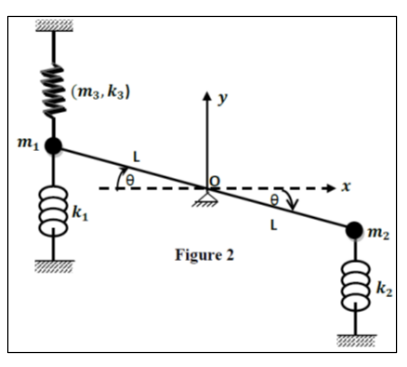
\includegraphics[width=0.7\textwidth]{images/vibrations/vib-001-000.png}
\caption{Système masse-ressort horizontal : schéma.}
\end{figure}

\begin{figure}[H]
\centering
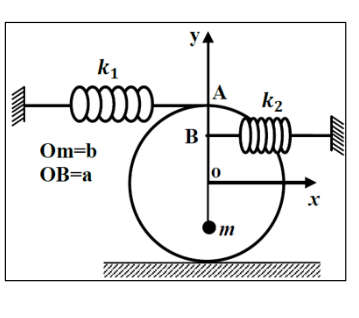
\includegraphics[width=0.7\textwidth]{images/vibrations/vib-002-004.png}
\caption{Poulie avec ressort et masse.}
\end{figure}

\begin{figure}[H]
\centering
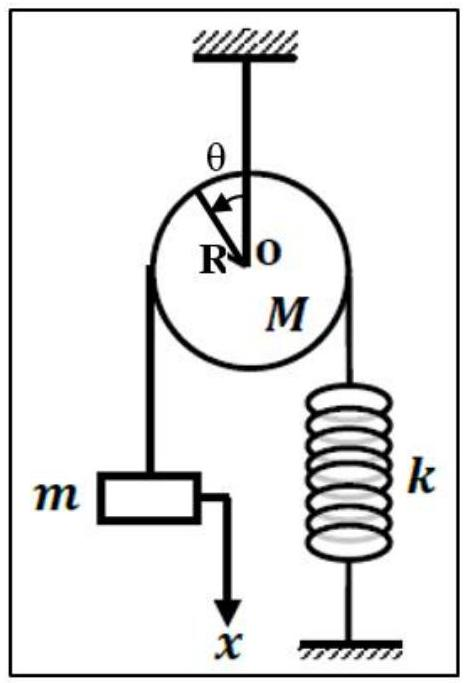
\includegraphics[width=0.7\textwidth]{images/vibrations/vib-004-007.png}
\caption{Oscillateur amorti : régime sous-critique.}
\end{figure}

\begin{figure}[H]
\centering
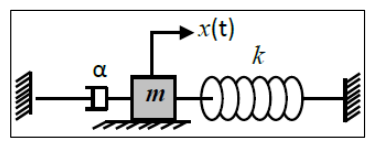
\includegraphics[width=0.7\textwidth]{images/vibrations/vib-006-008.png}
\caption{Résonance d'un oscillateur forcé.}
\end{figure}

\begin{figure}[H]
\centering
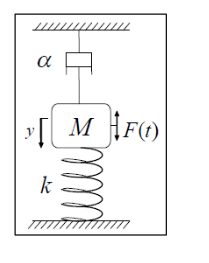
\includegraphics[width=0.7\textwidth]{images/vibrations/vib-009-014.png}
\caption{Deux masses couplées par un ressort.}
\end{figure}

\begin{figure}[H]
\centering
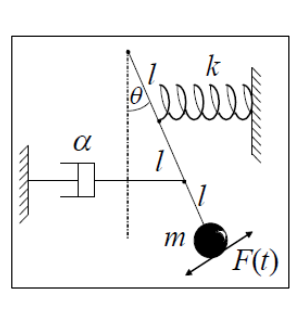
\includegraphics[width=0.7\textwidth]{images/vibrations/vib-011-016.png}
\caption{Modes normaux d'un système à 2 ddl.}
\end{figure}

\begin{figure}[H]
\centering
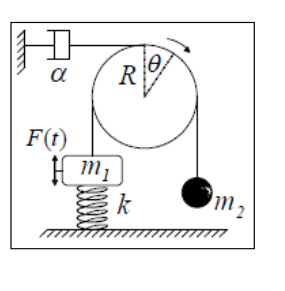
\includegraphics[width=0.7\textwidth]{images/vibrations/vib-013-018.png}
\caption{Barre oscillante avec amortissement.}
\end{figure}

\begin{figure}[H]
\centering
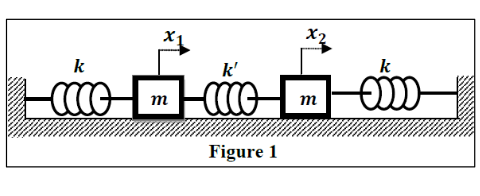
\includegraphics[width=0.7\textwidth]{images/vibrations/vib-015-020.png}
\caption{Ondes progressives sur une corde.}
\end{figure}

\begin{figure}[H]
\centering
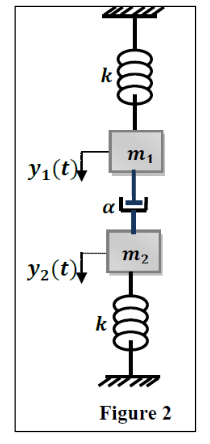
\includegraphics[width=0.7\textwidth]{images/vibrations/vib-017-022.png}
\caption{Ondes stationnaires : n\oe{}uds et ventres.}
\end{figure}

\begin{figure}[H]
\centering
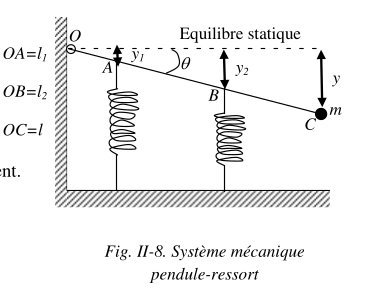
\includegraphics[width=0.7\textwidth]{images/vibrations/vib-018-024.png}
\caption{Battements : somme de deux oscillations.}
\end{figure}

\begin{figure}[H]
\centering
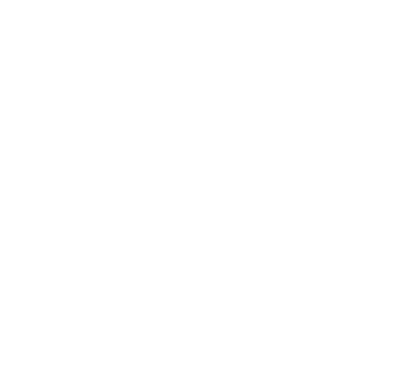
\includegraphics[width=0.7\textwidth]{images/vibrations/vib-001-001.png}
\caption{Pendule simple : mise en équation.}
\end{figure}

\begin{figure}[H]
\centering
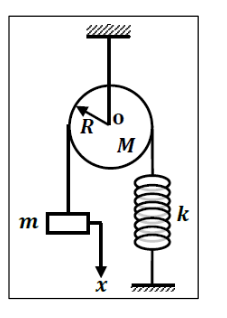
\includegraphics[width=0.7\textwidth]{images/vibrations/vib-001-002.png}
\caption{Pendule élastique vertical.}
\end{figure}

\begin{figure}[H]
\centering
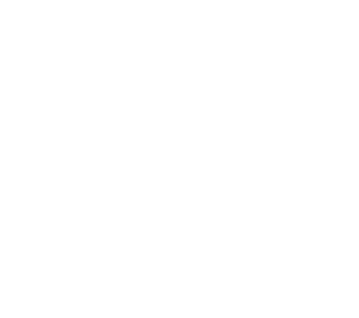
\includegraphics[width=0.7\textwidth]{images/vibrations/vib-002-005.png}
\caption{Oscillateur amorti : régime apériodique.}
\end{figure}

\begin{figure}[H]
\centering
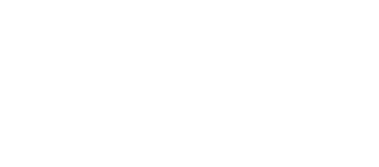
\includegraphics[width=0.7\textwidth]{images/vibrations/vib-006-009.png}
\caption{Résonance en force d'un oscillateur harmonique.}
\end{figure}

\begin{figure}[H]
\centering
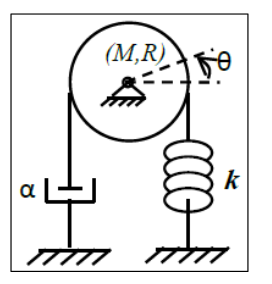
\includegraphics[width=0.7\textwidth]{images/vibrations/vib-006-010.png}
\caption{Bande passante et facteur de qualité.}
\end{figure}

\begin{figure}[H]
\centering
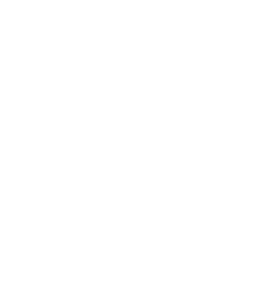
\includegraphics[width=0.7\textwidth]{images/vibrations/vib-006-011.png}
\caption{Oscillations couplées : modes normaux.}
\end{figure}

\begin{figure}[H]
\centering
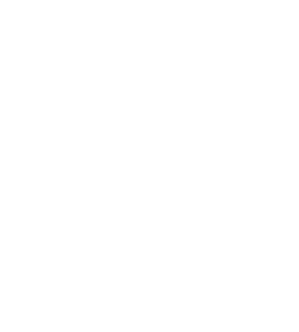
\includegraphics[width=0.7\textwidth]{images/vibrations/vib-011-017.png}
\caption{Couplage par ressort entre deux masses.}
\end{figure}

\begin{figure}[H]
\centering
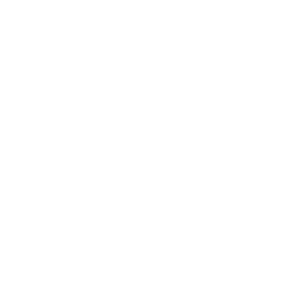
\includegraphics[width=0.7\textwidth]{images/vibrations/vib-013-019.png}
\caption{Système à trois masses couplées.}
\end{figure}

\begin{figure}[H]
\centering
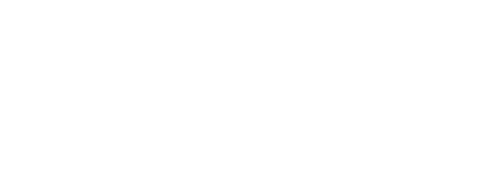
\includegraphics[width=0.7\textwidth]{images/vibrations/vib-015-021.png}
\caption{Corde vibrante : équation d'Alembert.}
\end{figure}

\begin{figure}[H]
\centering
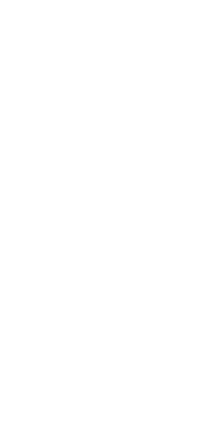
\includegraphics[width=0.7\textwidth]{images/vibrations/vib-017-023.png}
\caption{Mode fondamental et harmoniques de corde.}
\end{figure}

\begin{figure}[H]
\centering
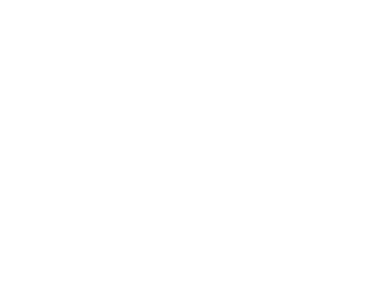
\includegraphics[width=0.7\textwidth]{images/vibrations/vib-018-025.png}
\caption{Analyse spectrale d'un signal en battements.}
\end{figure}

\ifdefined\inMainDoc\else\end{document}\fi
